\documentclass[a4paper,10pt,twocolumn]{ltjarticle}
\usepackage{kaitoushu}

% グラフ用の共通スタイル定義
\pgfplotsset{
  myaxis/.style={
    axis lines=middle,
    xlabel={$x$}, ylabel={$y$},
    every axis x label/.style={at={(ticklabel* cs:1)},anchor=west},
    every axis y label/.style={at={(ticklabel* cs:1)},anchor=south},
    tick label style={font=\scriptsize},
    label style={font=\small},
    width=5.5cm, height=5cm,
    grid=none,
    samples=100,
  }
}

\begin{document}

\problemrange{3章：関数とグラフ — Basic (p.31)（問143--155）}



\mondai{143}{$f(x)=3x+1$ のとき，$f(2)$，$f(-2)$，$f(a+2)$，$f(a-2)$ を求めよ．}
\kotae{
関数の値を求めるには，$f(x)=3x+1$ の $x$ に指定された値をそのまま代入する．

(1) $f(2)=3\cdot2+1=6+1=7$

(2) $f(-2)=3\cdot(-2)+1=-6+1=-5$

(3) $x$ に $a+2$ をカッコごと代入：
$f(a+2)=3(a+2)+1=3a+6+1=3a+7$

(4) 同様に $x$ に $a-2$ を代入：
$f(a-2)=3(a-2)+1=3a-6+1=3a-5$
}

\mondai{144}{次の関数の（\quad）内の定義域に対する値域を求めよ．}
\kotae{
1次関数の値域は，定義域の両端での値を調べればよい．

(1) $y=2x+1\;(-1\leqq x\leqq 2)$

傾き $2>0$（単調増加）．
$x=-1$：$y=-1$，$x=2$：$y=5$

$\therefore -1\leqq y\leqq 5$

(2) $y=-2x+4\;(-1\leqq x\leqq 1)$

傾き $-2<0$（単調減少）．
$x=-1$：$y=6$，$x=1$：$y=2$

$\therefore 2\leqq y\leqq 6$
}

\mondai{145}{次の関数のグラフをかけ．また，軸と頂点の座標を求めよ．}
\kotae{
$y=a(x-p)^{2}+q$ の形から，軸 $x=p$，頂点 $(p,q)$．
$a>0$：下に凸，$a<0$：上に凸．

(1) $y=x^{2}-1$\quad 軸：$x=0$，頂点：$(0,-1)$

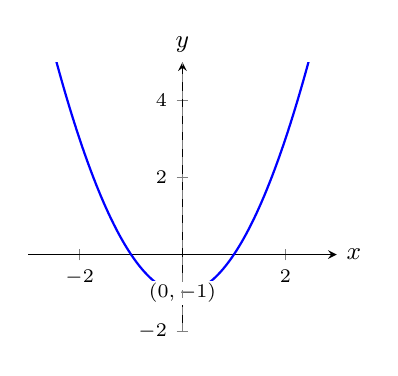
\begin{tikzpicture}
\begin{axis}[myaxis, xmin=-3,xmax=3,ymin=-2,ymax=5]
\addplot[thick,blue,domain=-2.5:2.5]{x^2-1};
\node[fill=white,inner sep=1pt,font=\scriptsize] at (axis cs:0,-1) {$(0,-1)$};
\addplot[dashed,gray] coordinates {(0,-2)(0,5)};
\end{axis}
\end{tikzpicture}

(2) $y=-(x-1)^{2}$\quad 軸：$x=1$，頂点：$(1,0)$

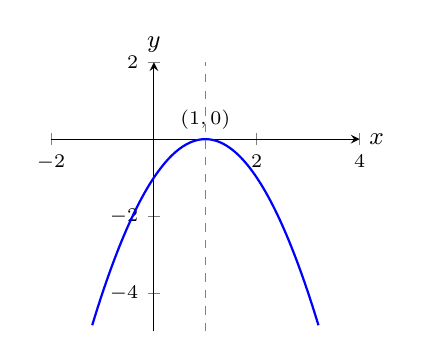
\begin{tikzpicture}
\begin{axis}[myaxis, xmin=-2,xmax=4,ymin=-5,ymax=2]
\addplot[thick,blue,domain=-1.2:3.2]{-(x-1)^2};
\node[fill=white,inner sep=1pt,font=\scriptsize] at (axis cs:1,0.5) {$(1,0)$};
\addplot[dashed,gray] coordinates {(1,-5)(1,2)};
\end{axis}
\end{tikzpicture}

(3) $y=3(x+1)^{2}-2$\quad 軸：$x=-1$，頂点：$(-1,-2)$

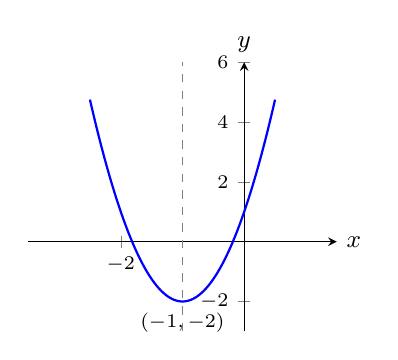
\begin{tikzpicture}
\begin{axis}[myaxis, xmin=-3.5,xmax=1.5,ymin=-3,ymax=6]
\addplot[thick,blue,domain=-2.5:0.5]{3*(x+1)^2-2};
\node[fill=white,inner sep=1pt,font=\scriptsize] at (axis cs:-1,-2.7) {$(-1,-2)$};
\addplot[dashed,gray] coordinates {(-1,-3)(-1,6)};
\end{axis}
\end{tikzpicture}

(4) $y=-\dfrac{1}{2}(x-2)^{2}+2$\quad 軸：$x=2$，頂点：$(2,2)$

\begin{tikzpicture}
\begin{axis}[myaxis, xmin=-1,xmax=5,ymin=-4,ymax=3]
\addplot[thick,blue,domain=-0.5:4.5]{-0.5*(x-2)^2+2};
\node[fill=white,inner sep=1pt,font=\scriptsize] at (axis cs:2,2.5) {$(2,2)$};
\addplot[dashed,gray] coordinates {(2,-4)(2,3)};
\end{axis}
\end{tikzpicture}
}

\mondai{146}{放物線 $y=2x^{2}$ を次のように平行移動した放物線の方程式を求めよ．}
\kotae{
平行移動の公式：$x$軸方向に$p$，$y$軸方向に$q$ → $y=2(x-p)^{2}+q$

(1) $x$軸方向に3：$y=2(x-3)^{2}$

(2) $x$方向に1，$y$方向に2：$y=2(x-1)^{2}+2$

(3) $x$方向に$-2$，$y$方向に$-1$：$y=2(x+2)^{2}-1$
}

\mondai{147}{次の2次関数を標準形に直し，グラフをかけ．}
\kotae{
\textbf{平方完成}の手順：$x^{2}$の係数でくくる → カッコ内を完成 → 整理．

(1) $y=x^{2}-2x+1=(x-1)^{2}$

軸：$x=1$，頂点：$(1,0)$

\begin{tikzpicture}
\begin{axis}[myaxis, xmin=-1.5,xmax=3.5,ymin=-1,ymax=5]
\addplot[thick,blue,domain=-0.8:2.8]{(x-1)^2};
\node[fill=white,inner sep=1pt,font=\scriptsize] at (axis cs:1,-0.6) {$(1,0)$};
\addplot[dashed,gray] coordinates {(1,-1)(1,5)};
\end{axis}
\end{tikzpicture}

(2) $y=2x^{2}-4x+3=2(x^{2}-2x)+3=2(x-1)^{2}+1$

軸：$x=1$，頂点：$(1,1)$

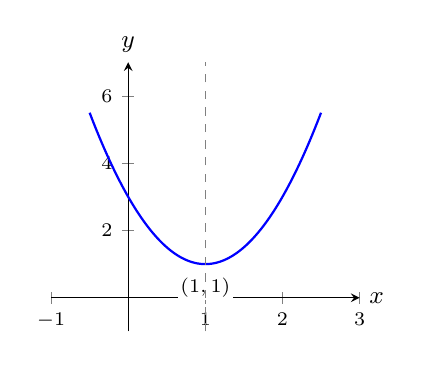
\begin{tikzpicture}
\begin{axis}[myaxis, xmin=-1,xmax=3,ymin=-1,ymax=7]
\addplot[thick,blue,domain=-0.5:2.5]{2*(x-1)^2+1};
\node[fill=white,inner sep=1pt,font=\scriptsize] at (axis cs:1,0.3) {$(1,1)$};
\addplot[dashed,gray] coordinates {(1,-1)(1,7)};
\end{axis}
\end{tikzpicture}

(3) $y=-x^{2}+4x-3=-(x-2)^{2}+1$

軸：$x=2$，頂点：$(2,1)$

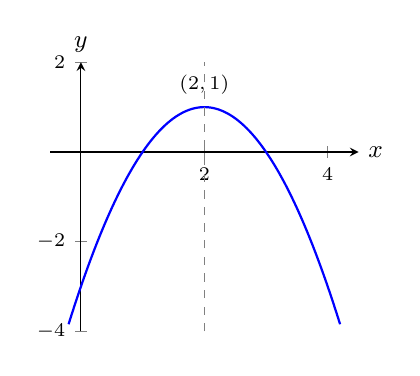
\begin{tikzpicture}
\begin{axis}[myaxis, xmin=-0.5,xmax=4.5,ymin=-4,ymax=2]
\addplot[thick,blue,domain=-0.2:4.2]{-(x-2)^2+1};
\node[fill=white,inner sep=1pt,font=\scriptsize] at (axis cs:2,1.5) {$(2,1)$};
\addplot[dashed,gray] coordinates {(2,-4)(2,2)};
\end{axis}
\end{tikzpicture}

(4) $y=x^{2}-x-2=\left(x-\dfrac{1}{2}\right)^{2}-\dfrac{9}{4}$

軸：$x=\dfrac{1}{2}$，頂点：$\left(\dfrac{1}{2},-\dfrac{9}{4}\right)$

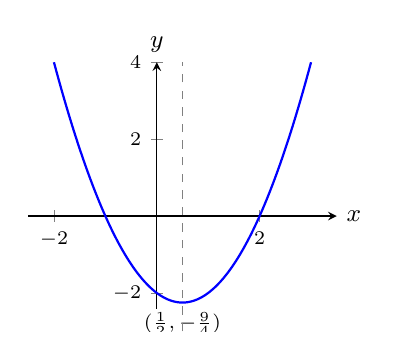
\begin{tikzpicture}
\begin{axis}[myaxis, xmin=-2.5,xmax=3.5,ymin=-3,ymax=4]
\addplot[thick,blue,domain=-2:3]{x^2-x-2};
\node[fill=white,inner sep=1pt,font=\scriptsize] at (axis cs:0.5,-2.8) {$(\frac{1}{2},-\frac{9}{4})$};
\addplot[dashed,gray] coordinates {(0.5,-3)(0.5,4)};
\end{axis}
\end{tikzpicture}

(5) $y=-\dfrac{1}{2}x^{2}+x=-\dfrac{1}{2}(x-1)^{2}+\dfrac{1}{2}$

軸：$x=1$，頂点：$(1,\frac{1}{2})$

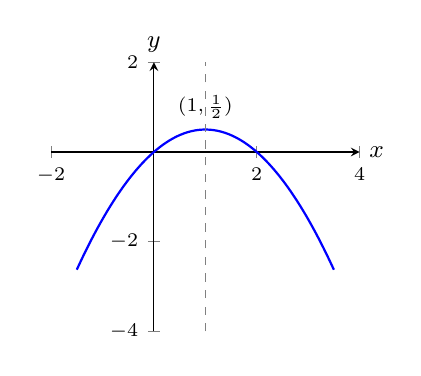
\begin{tikzpicture}
\begin{axis}[myaxis, xmin=-2,xmax=4,ymin=-4,ymax=2]
\addplot[thick,blue,domain=-1.5:3.5]{-0.5*x^2+x};
\node[fill=white,inner sep=1pt,font=\scriptsize] at (axis cs:1,1) {$(1,\frac{1}{2})$};
\addplot[dashed,gray] coordinates {(1,-4)(1,2)};
\end{axis}
\end{tikzpicture}

(6) $y=-2x^{2}-3x+2=-2\!\left(x+\dfrac{3}{4}\right)^{2}+\dfrac{25}{8}$

軸：$x=-\dfrac{3}{4}$，頂点：$\left(-\dfrac{3}{4},\dfrac{25}{8}\right)$

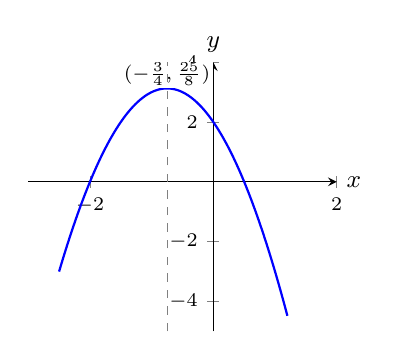
\begin{tikzpicture}
\begin{axis}[myaxis, xmin=-3,xmax=2,ymin=-5,ymax=4]
\addplot[thick,blue,domain=-2.5:1.2]{-2*x^2-3*x+2};
\node[fill=white,inner sep=1pt,font=\scriptsize] at (axis cs:-0.75,3.6) {$(-\frac{3}{4},\frac{25}{8})$};
\addplot[dashed,gray] coordinates {(-0.75,-5)(-0.75,4)};
\end{axis}
\end{tikzpicture}
}

\mondai{148}{2次関数 $y=a(x-p)^{2}+q$ で表される放物線で，次の条件を満たすものを求めよ．}
\kotae{
頂点や軸の情報から式の骨格を作り，通る点を代入して未知数を求める．

(1) 頂点$(3,5)$ → $y=a(x-3)^{2}+5$．

$(0,-4)$ 代入：$-4=9a+5$，$a=-1$

$\therefore y=-(x-3)^{2}+5$

(2) 頂点が$y$軸上 → $y=ax^{2}+q$．

$(-1,1)$：$a+q=1\;\cdots$①\quad $(2,-5)$：$4a+q=-5\;\cdots$②

②$-$①：$3a=-6$，$a=-2$，$q=3$ → $y=-2x^{2}+3$

(3) 軸$x=2$ → $y=a(x-2)^{2}+q$．

$(0,5)$：$4a+q=5$\quad $(3,2)$：$a+q=2$

$3a=3$，$a=1$，$q=1$ → $y=(x-2)^{2}+1$
}

\mondai{149}{次の条件を満たし，$y$軸に平行な軸をもつ放物線の方程式を求めよ．また，軸と頂点を求め，グラフをかけ．}
\kotae{
(1) 3点$(1,0)$，$(0,3)$，$(2,-1)$を通る．

$y=ax^{2}+bx+c$．$c=3$，$a+b=-3$，$2a+b=-2$

$a=1$，$b=-4$．$y=x^{2}-4x+3=(x-2)^{2}-1$

軸：$x=2$，頂点：$(2,-1)$

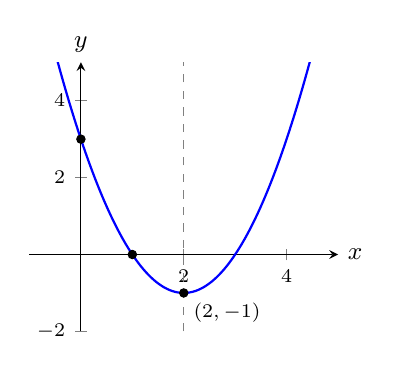
\begin{tikzpicture}
\begin{axis}[myaxis, xmin=-1,xmax=5,ymin=-2,ymax=5]
\addplot[thick,blue,domain=-0.5:4.5]{x^2-4*x+3};
\addplot[only marks,mark=*,mark size=1.5pt] coordinates {(1,0)(0,3)(2,-1)};
\node[font=\scriptsize,right] at (axis cs:2,-1.5) {$(2,-1)$};
\addplot[dashed,gray] coordinates {(2,-2)(2,5)};
\end{axis}
\end{tikzpicture}

(2) $x$軸と$(3,0)$，$(-2,0)$で交わり，$y$軸と$(0,6)$で交わる．

$y=a(x-3)(x+2)$．$(0,6)$：$-6a=6$，$a=-1$

$y=-(x-3)(x+2)=-x^{2}+x+6=-\!\left(x-\dfrac{1}{2}\right)^{2}+\dfrac{25}{4}$

軸：$x=\dfrac{1}{2}$，頂点：$\left(\dfrac{1}{2},\dfrac{25}{4}\right)$

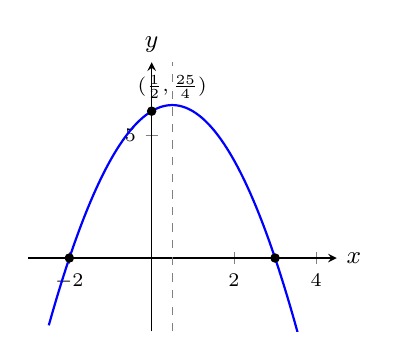
\begin{tikzpicture}
\begin{axis}[myaxis, xmin=-3,xmax=4.5,ymin=-3,ymax=8]
\addplot[thick,blue,domain=-2.5:3.8]{-x^2+x+6};
\addplot[only marks,mark=*,mark size=1.5pt] coordinates {(3,0)(-2,0)(0,6)};
\node[font=\scriptsize] at (axis cs:0.5,7) {$(\frac{1}{2},\frac{25}{4})$};
\addplot[dashed,gray] coordinates {(0.5,-3)(0.5,8)};
\end{axis}
\end{tikzpicture}
}

\mondai{150}{次の2次関数の最大値または最小値を求めよ．}
\kotae{
$a>0$（下に凸）→ 頂点で最小値，$a<0$（上に凸）→ 頂点で最大値．

(1) $y=(x-2)^{2}+4$\quad $x=2$ で最小値 $4$

(2) $y=-(x-3)^{2}+8$\quad $x=3$ で最大値 $8$

(3) $y=\dfrac{1}{2}(x-2)^{2}-2$\quad $x=2$ で最小値 $-2$

(4) $y=-3(x-1)^{2}+5$\quad $x=1$ で最大値 $5$
}

\mondai{151}{次の関数について，（\quad）内の定義域における最大値と最小値を求めよ．}
\kotae{
手順：① 平方完成 → ② 頂点が定義域内か判定 → ③ 端と頂点を比較．

(1) $y=(x-2)^{2}-4\;(0\leqq x\leqq 3)$

$x=0$：$0$，$x=2$：$-4$，$x=3$：$-3$

最小値 $-4$（$x=2$），最大値 $0$（$x=0$）

(2) $y=(x-3)^{2}-2\;(0\leqq x\leqq 2)$

頂点$x=3$は域外．単調減少．$x=0$：$7$，$x=2$：$-1$

最小値 $-1$（$x=2$），最大値 $7$（$x=0$）

(3) $y=-(x-1)^{2}+3\;(-1\leqq x\leqq 1)$

$x=-1$：$-1$，$x=1$：$3$

最小値 $-1$（$x=-1$），最大値 $3$（$x=1$）

(4) $y=2(x-2)^{2}-3\;(0\leqq x\leqq 4)$

$x=0$：$5$，$x=2$：$-3$，$x=4$：$5$

最小値 $-3$（$x=2$），最大値 $5$（$x=0,4$）

(5) $y=-\dfrac{1}{2}(x+1)^{2}+\dfrac{7}{2}\;(-2\leqq x\leqq 2)$

$x=-2$：$3$，$x=-1$：$\dfrac{7}{2}$，$x=2$：$-1$

最小値 $-1$（$x=2$），最大値 $\dfrac{7}{2}$（$x=-1$）

(6) $y=2\!\left(x-\dfrac{3}{2}\right)^{2}-\dfrac{1}{2}\;(0\leqq x\leqq 2)$

$x=0$：$4$，$x=\dfrac{3}{2}$：$-\dfrac{1}{2}$，$x=2$：$0$

最小値 $-\dfrac{1}{2}$（$x=\dfrac{3}{2}$），最大値 $4$（$x=0$）
}

\mondai{152}{底辺の長さと高さの和が8\,cmである三角形の底辺の長さを$x$\,cmとするとき，三角形の面積が最大となる$x$の値とその最大値を求めよ．}
\kotae{
底辺$x$，高さ$(8-x)$（$0<x<8$）．

$S=\dfrac{1}{2}x(8-x)=-\dfrac{1}{2}(x-4)^{2}+8$

$x=4$ のとき最大値 $S=8$\,cm$^{2}$
}

\mondai{153}{次の2次関数のグラフと$x$軸との共有点を調べよ．また，共有点をもつときは，その$x$座標を求めよ．}
\kotae{
$y=0$ とおいた方程式の判別式 $D$ で判定．

(1) $2x^{2}+5x+1=0$：$D=17>0$ → 2点

$x=\dfrac{-5\pm\sqrt{17}}{4}$

(2) $3x^{2}-7x+5=0$：$D=-11<0$ → 共有点なし

(3) $\dfrac{1}{3}x^{2}-2x+3=0$ → $x^{2}-6x+9=(x-3)^{2}=0$

$D=0$ → 接する．$x=3$
}

\mondai{154}{次の2次関数のグラフが（\quad）内の条件を満たすように，定数$k$の値または値の範囲を定めよ．}
\kotae{
(1) $y=x^{2}+3x+k$（2点で交わる）

$D=9-4k>0$ → $k<\dfrac{9}{4}$

(2) $y=4x^{2}-2kx+9$（接する）

$D=4k^{2}-144=0$ → $k=\pm6$

(3) $y=kx^{2}+x-1$（共有点なし）

$k=0$は不適．$k\neq0$：$D=1+4k<0$ → $k<-\dfrac{1}{4}$
}

\mondai{155}{次の2次不等式を解け．}
\kotae{
(1) $(x+1)(x+3)\geqq0$ → $x\leqq-3$ または $x\geqq-1$

(2) $x=1\pm\sqrt{2}$ → $1-\sqrt{2}<x<1+\sqrt{2}$

(3) $(x-3)^{2}>0$ → $x\neq3$ のすべての実数

(4) $(2x-3)^{2}<0$ → 解なし

(5) $\left(x-\dfrac{1}{2}\right)^{2}\geqq0$ → すべての実数

(6) $(x-4)^{2}\leqq0$ → $x=4$

(7) $4x^{2}-6x+3>0$，$D<0$で常に正 → すべての実数

(8) $D<0$で常に正 → 解なし
}

\end{document}
